% !TEX root = thesis.tex

\setlength{\epigraphwidth}{0.85\textwidth}
\epigraph{In the winter of 1867-1868 I observed the auroral spectrum several times. A single bright spectral line is never absent in auroral light. I determined the wavelength of this line to be \unit[5567]{\AA}.}{\citep{angstrom1869}}

\graphicspath{{Intro/}}
Aurora is a useful ``gateway drug'' for getting the general populace interested in supporting and even participating in geoscience.
The fanciful varying forms of aurora fascinated northern prehistoric tribes living within view of the auroral oval (typically $60^\circ..70^\circ$N).
Those living in mid-latitudes well below $60^\circ$N were also fascinated and frightened by the infrequent appearance of aurora we now know to be correlated with the expansion of the auroral oval due to strong solar activity.
The spherical asymmetry of the geomagnetic field puts the southern auroral oval over Antarctica and the Southern Ocean, regions suffering from a lack of targeted scientific inquiry until the dawn of the twentieth century \citep{davies1931}. 
Spatiotemporally fine structured aurora is well-known to be caused by Alfvén wave breaking along geomagnetic field lines of ionospheric particles.
%...''wave breaking'' instead of acceleration per jls 1/6/17
In the past decade, targeted studies associating naturally enhanced ion acoustic lines (NEIALs) began in earnest \citep{michell2005}, and the instruments, algorithms and observations encapsulated in the dissertation represent the latest step in this chain of inquiry.

More than 2400 years before \citet{angstrom1869} measured with 0.18\% error the bright yellow-green \unit[5577]{\AA} auroral emission line, punctilious Babylonian astronomers recorded the earliest datable auroral event on March 12, 587~BCE \citep{stephenson2004}.
Auroral observational records are at least dense enough to extend solar cycle estimates back to the second century BCE \citep{stothers1979}, with scattered records reaching back a few centuries further \citep{siscoe2002,silverman2006}.
Simultaneous independent observations of auroral events (first known to occur January 31, 1101) were repeated numerous times in following centuries throughout the Northern Hemisphere \citep{willis1999}.
The first recorded auroral conjugacy was on September 16, 1770 with observers in China and the ocean north of the Australian coast \citep{willis1996} as depicted in Figure~\ref{fig:firstconj}.
\begin{figure}\centering
    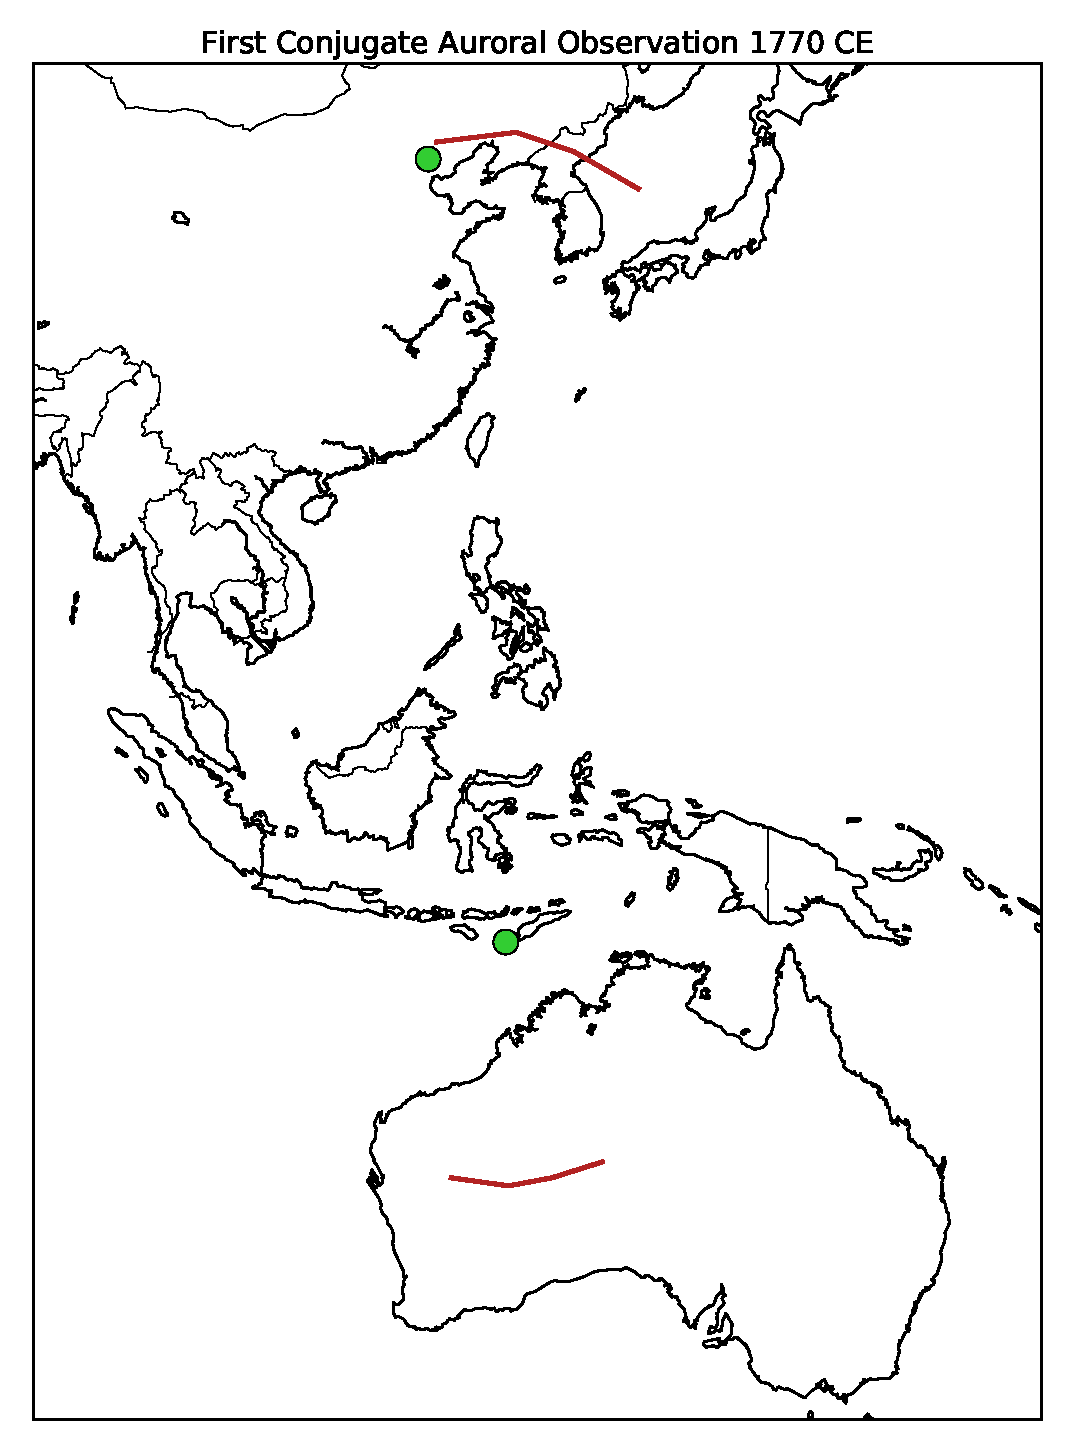
\includegraphics[width=0.8\linewidth]{gfx/firstconj}
    \caption{First recorded simultaneous auroral conjugate observation: September 16, 1770. Green circles represent observer locations. Red arcs indicate modeled location of \unit[630]{nm} forbidden [OI]21 auroral emissions \citep{willis1996}.}\label{fig:firstconj}
\end{figure}
The oldest observations record primarily red emissions more common at mid-latitudes driven by powerful solar storms greatly expanding the auroral oval over populated areas \citep{silverman1998}.

Nineteenth century auroral research included estimates of the height and shape of the aurora \citep{omholtbook}, which researchers in the twentieth century would recognize as proxies for the magnetospheric mechanisms driving the aurora.
Detailed records from South Asia and East Asia during and after the 1859 Carrington Event \citep{hayakawa2016east,keika2015caused} have allowed scientific speculation on what might be observed with contemporary instruments.
The pair of late nineteenth century auroral sketches in Figure~\ref{fig:chernouss6} \citep{chernouss2005} show an example of the opportunity and difficulty in extracting science quantities from ground observations of aurora due to perspective effects of the optically thin aurora.
That is, the observed brightness of aurora is equal to the line integral along the line of sight--stars are plainly seen through the aurora.
\begin{figure}\centering
    \begin{subfigure}[t]{0.45\linewidth}\centering
        \includegraphics[width=\linewidth]{gfx/chernouss6a}
        \caption{Auroral arc sketched from below.}\label{fig:1a}		
    \end{subfigure}
    \begin{subfigure}[t]{0.45\linewidth}\centering
        \includegraphics[width=\linewidth]{gfx/chernouss6b}
        \caption{Auroral arc sketched from oblique perspective.}\label{fig:1b}		
    \end{subfigure}
    \caption{Nineteenth century scientific auroral sketch by J. Sýkora \citep{chernouss2005}. 
    	In a typical case, two simultaneous observers, one beneath the arc would sees panel (a) and another observer $\sim \unit[100]{km}$ away sees panel (b).}
    \label{fig:chernouss6}
\end{figure}
Descriptions of aurora as rayed, striped, curtained, \&c. extend from the seventeenth century through the present.
Such terms are strongly biased by observer location, as lateral displacement of several kilometers can yield a rather different description of the same auroral form as discussed in \citet{semeter2012} and as modeled in Figure~\ref{fig:camres}.
Attempts to establish auroral heights presented great difficulty through the mid-1800s, with auroral altitude estimates spanning \unit[7..1100]{km} \citep{schwickert1833}.
Advances of the telegraph allowed distant synchronized photographs to be taken, and star registration techniques in part proposed by \citet{schwickert1833} were finally implemented by \citet{stormer1930} allowing plausible estimates of auroral height.

This dissertation describes the latest advances in joint studies of Langmuir turbulence associated with structured aurora using Incoherent Scatter Radar (ISR) and a network of synchronized cameras.
A schematic diagram \citep{schunk2006} of ionospheric features relevant to this dissertation is given in Figure~\ref{fig:aeroiono}.
\begin{figure}\centering
    \includegraphics[width=0.5\linewidth,trim=0 0 340 50,clip]{gfx/aeroiono}
    \caption{Ionospheric layers (from \citet{schunk2006})}\label{fig:aeroiono}
\end{figure}
The D-layer of the ionosphere lies from about 60..\unit[90]{km} and is a daytime only phenomenon due to intense short-wavelength UV bombardment from the sun, with the electron density enhancement quickly disappearing after sunset.
The E-layer of the ionosphere lies from approximately 90..\unit[150]{km} and is the altitude region where most finely structured aurora exists.
The F-layer of the ionosphere extends from \unit[150]{km} to several hundred km altitude. 
This dissertation discusses each of these elements in context and their connection to next generation instruments already being built.
